\section{Implementation of the Experiment}
\label{sec:Durchführung}
To observe and record the Rubidum absoptionspectrum at the end
of the experiment
serveral premeasurements with different setups are necessary.
% Used devices are two Photodiodes and
% of cause a diode laser
A dark room for the experiment is recommended to minize the
interfering light sources.
The used diode laser has two knobs to controll the alignment of grating
as shown in figure \ref{fig:knobs}.
For the horizontal alignment the side knob is turned. The
top knob changes the vertical alignment.
\begin{figure}
  \centering
  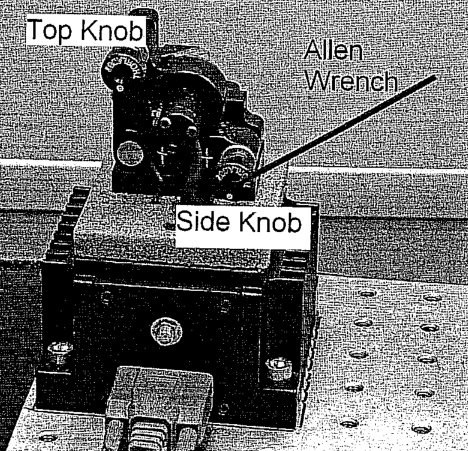
\includegraphics[width=0.7\textwidth]{Laserknobs.png}
  \caption{It is shown top knob and side knob of the diode laser to align the grating.\cite{V61}}
  \label{fig:knobs}
\end{figure}


\subsection{Setup and Procedure}
\label{subsec:setup}
The fist step is to determine the threshold current
of the diode laser.
Therefore an index card is placed in front of the laser beam and the CCD Camera
is focused on the point where the card intercpets the beam.
The setup is displayed
in figure \ref{fig:setup1}.

\begin{figure}
  \centering
  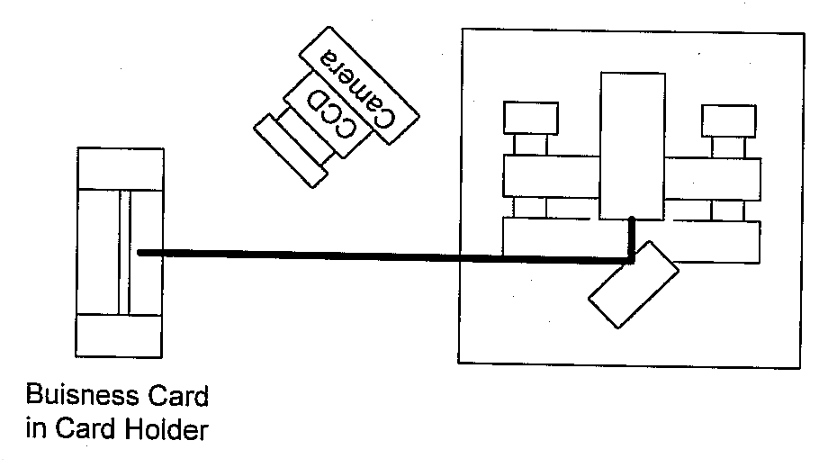
\includegraphics[width=0.7\textwidth]{setup1.png}
  \caption{Schematical setup to observe the threshold current of the diode laser.\cite{V61}}
  \label{fig:setup1}
\end{figure}
By increasing the current, starting at zero, the transition from
a normal LED to a laser diode is observed.
The threshold current is at the
transition point where the light spot becomes significantly brighter.
Futhermore by adjusting the top knob the threshold current can be lowered.

% The thresholf current can verrigert werden durch
%( irgendwas mit den Rädchen)

After the lowest possible threshold current is determined, the
index card is removed and
the rubidum absorption cell
is placed in the laserbeam instead.
A schematical setup is shown in figure \ref{fig:setup2}
Additionally the diode laser's ramp generator and  piezo controller is wired as shown in figure \ref{fig:dl_controll}.
The camera is now
focused on the absorption cell and
the diode is set to operate above the threshold current.
\begin{figure}
  \centering
  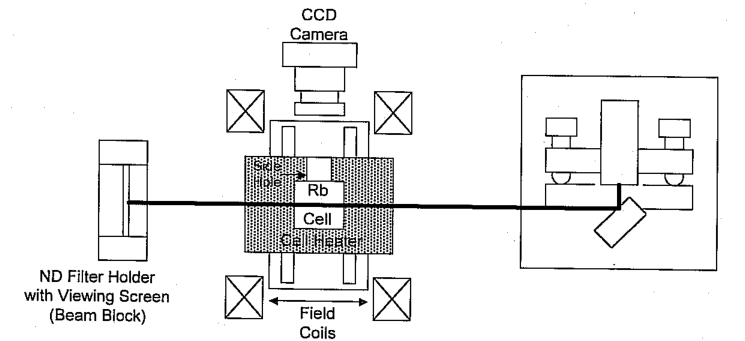
\includegraphics[width=0.7\textwidth]{setup2.png}
  \caption{Schematical setup to observe the Rubidium florescence.\cite{V61}}
  \label{fig:setup2}
\end{figure}

\begin{figure}
  \centering
  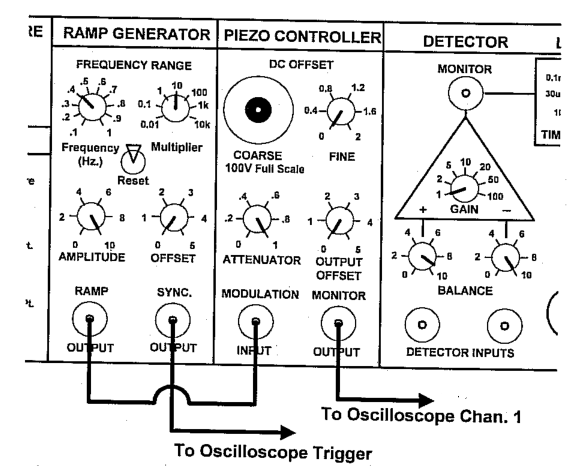
\includegraphics[width=0.7\textwidth]{wiring.png}
  \caption{Wiring of the piezo controlelement to observe the Rubidium fluorescence.\cite{V61}}
  \label{fig:dl_controll}
\end{figure}

By adjusting the side knob and the current,
the fluorescence of Rb atoms in the absorption cell
can be observed
as a fluorescence flashing along the laserbeam.
Besides the observation with the camera a photodiode,
which measures the intensity
of the outgoing laserbeam,
is installed behind the absoption cell and
connected to an oscilloscope to
see some fraction of the Rubidum absorption spectrum .

To achieve the visualisation of the full Rubidum
spectrum
simultaneous current and piezo modulation
is necessary. Therefore the ramp generator output
is connected also to the current modulation input.
With some adjustments of the current and the side knob
??a full trance over the Rubidum is displayed at the  oscilloscope.

A second method to obtain the absoptionspectrum
is as follows.
The setup of the other method is shown in
figure \ref{fig:setup3}.
Additionally to the setup before a beam splitter is added
betweeen diode laser and Rubidum cell.
A second photodiode is installed in the splitted laser beam of the beam splitter
in order to optian a signal without the Rubidum absoption spectrum.
The different signals of the two photondiodes are send to the
laser controller as shown in figure \ref{fig:dl_controll2}.
Since output of the operational amplifier is
the  difference between the two signals,
only the rubidum absoption and not the signal of the ramp generator is
displayed with the oscilloscope.

\begin{figure}
  \centering
  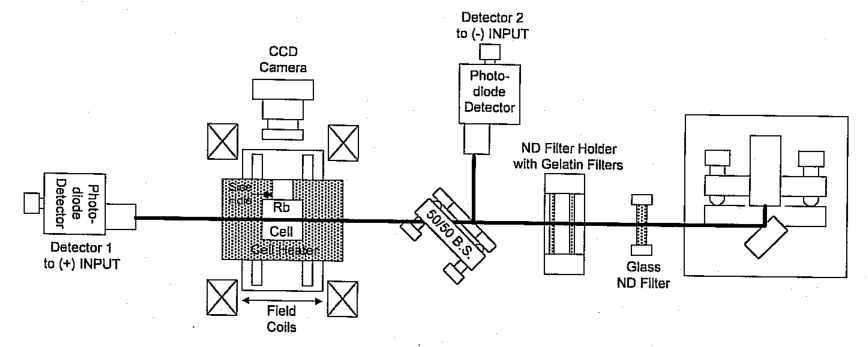
\includegraphics[width=0.7\textwidth]{setup3.png}
  \caption{Another schematical setup to observe the Rubidium absoptionspectrum.\cite{V61}}
  \label{fig:setup3}
\end{figure}


\begin{figure}
  \centering
  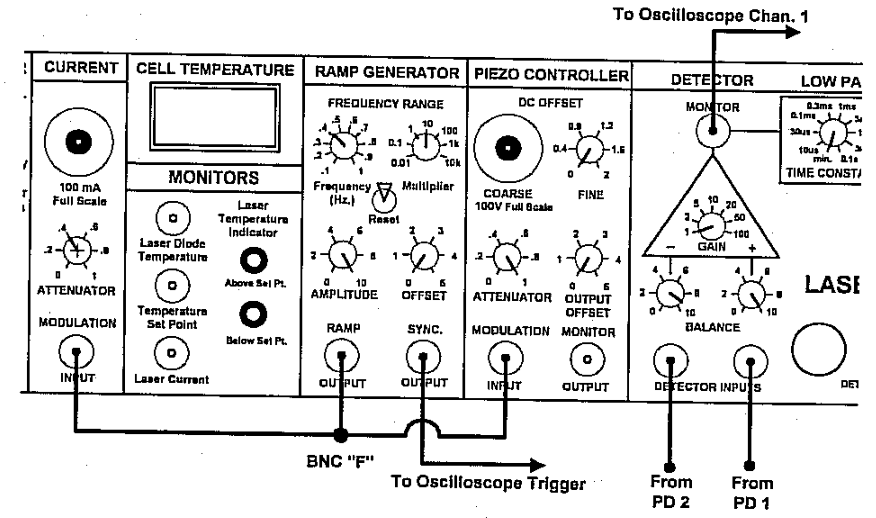
\includegraphics[width=0.7\textwidth]{wiring2.png}
  \caption{Wiring of the controllelement to observe the Rubidium florescence.\cite{V61}}
  \label{fig:dl_controll2}
\end{figure}
